\documentclass[]{agujournal2019}
\usepackage{url} %this package should fix any errors with URLs in refs.
\usepackage{lineno}
\usepackage[inline]{trackchanges} %for better track changes. finalnew option will compile document with changes incorporated.
\usepackage{soul}
\linenumbers

\usepackage{color}
\newcommand*{\todo}[1]{\textbf{\textcolor{red}{(#1)}}}

% Goes against template but looks a lot nicer.
\justifying 

% To mark revisions:
%
%  \note[editor]{The note}
%  \annote[editor]{Text to annotate}{The note}
%  \add[editor]{Text to add}
%  \remove[editor]{Text to remove}
%  \change[editor]{Text to remove}{Text to add}

\draftfalse
\journalname{Geophysical Research Letters}

\begin{document}

\title{Changes in damaging hail in major Australian cities with global warming}

\authors{Timothy H. Raupach\affil{1,2,3}, Joanna Aldridge\affil{4,5}}

\affiliation{1}{UNSW Institute for Climate Risk and Response, 
                UNSW Sydney, New South Wales, Australia}
\affiliation{2}{UNSW Climate Change Research Centre, 
                UNSW Sydney, New South Wales,  Australia}
\affiliation{3}{ARC Centre of Excellence for Climate Extremes, 
                Sydney, New South Wales,  Australia}
\affiliation{4}{School of Geosciences, University of Sydney, 
                Sydney, New South Wales,  Australia}
\affiliation{5}{QBE Australia, Sydney, 
                New South Wales, Australia}

\correspondingauthor{Timothy H. Raupach}{timothy.h.raupach@gmail.com}

\begin{keypoints}
\item \todo{Point 1}
\item \todo{Point 2}
\item \todo{Point 3}
\end{keypoints}

\begin{abstract}
      \todo{Abstract\ldots}
\end{abstract}

\section*{Plain Language Summary}
\todo{Plain language summary\ldots}

\section{Introduction}

\section{Methods}

\subsection{Simulations of historical and projected weather}

Historical and future simulations were produced using the Advanced Research Weather Research and Forecasting (AR-WRF) weather model version 4.4.1 \cite{Skamarock_2021} for four nested domains covering major Australian cities. We used one coarse- ($\sim$27 km grid spacing), two medium- ($\sim$9 km), and four fine-resolution ($\sim$3 km) domains with a parent-child scaling ratio of three. The model domains are shown in Figure \ref{fig:domains} and parameterisation schemes used are shown in Table \ref{tab:schemes}. The timestep for the coarse domain was set to 100 s, but reduced to 80 s or 60 s for simulation days on which Courant-Friedrichs-Lewy (CFL) errors occurred \todo{see comment in Section \ref{sec:results}}. WRF-HAILCAST \cite{Adams-Selin_WF_2019} was enabled for the fine-resolution domains, to estimate maximum hailstone diameters at the surface between each hourly output. Simulations were run for two scenarios of 20 convective seasons each: the historical scenario ran from 1989 to 2009, and the future scenario from 2080 to 2100. For each convective season, simulations were run from September 30 to February 28 inclusive, with hourly output resolution, and the first 24 hours of each season were discarded as model spin-up time. Boundary condition inputs were prepared using the \texttt{nc2wrf} code of \citeA{Xu_code_data_2021}. 

\begin{figure}[h!]
      \noindent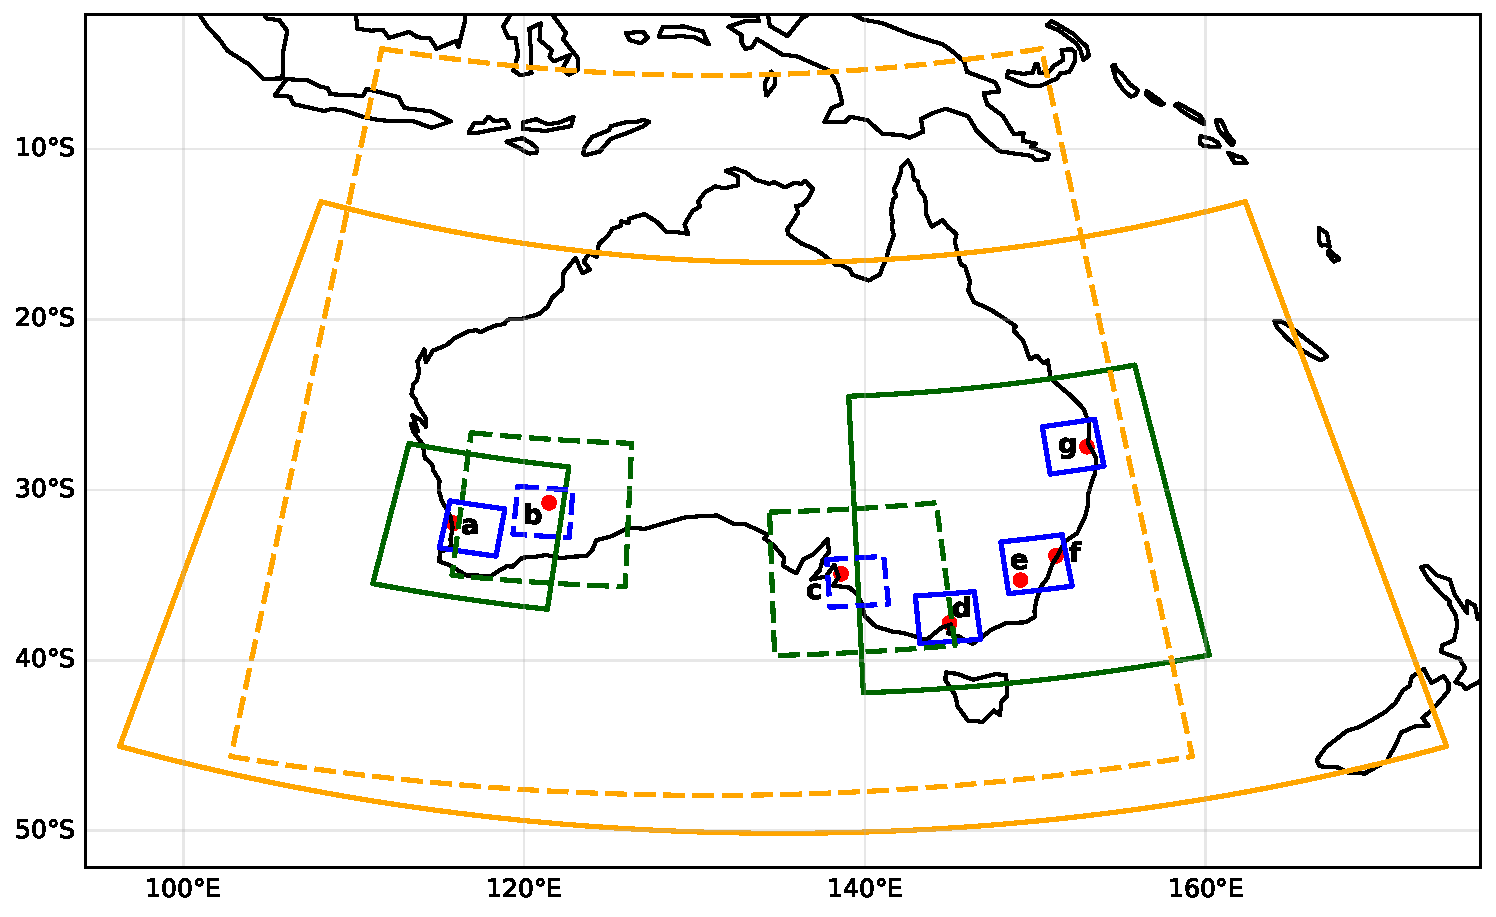
\includegraphics[width=\textwidth]{figures/domains}
      \caption{Approximate extents of the model domains on a map of Australia. The coarse-resolution domain is in yellow, medium-resolution domains in dark green, and fine-resolution domains in blue. Approximate city locations (with city extents not shown) are marked with red points for a) Perth, b) Melbourne, c) Canberra, d) Sydney, and e) Brisbane.}
      \label{fig:domains}
\end{figure}

\begin{table}[h!]
\caption{Parameterisation schemes used in the WRF simulations.}
\label{tab:schemes}
\centering
\begin{tabular}{lr}
      \hline
      Microphysics & P3-3moment \cite{Milbrandt_JAS_2021} \\
      Cumulous (medium and coarse nests only) & New Tiedtke \cite{Zhang_JC_2017} \\
      Longwave and shortwave radiation & RRTMG \cite{Iacono_JGRA_2008} \\
      Planetary boundary layer & YSU \cite{Hong_MWR_2006} \\
      Surface layer & Revised MM5 \cite{Jimenez_MWR_2012} \\
      Land surface & Noah-MP \cite{Niu_JGRA_2011} \\
      \hline
\end{tabular}
\end{table}

\subsection{Data preprocessing}

\subsection{Statistical modelling of extreme values}

Modelling of extreme values was done using the R \cite{R_software} package \texttt{extRemes} \cite{Gilleland_JSS_2016}. Block maxima were defined as daily maximum hailstone size per domain, under the assumption that such a timeseries would be close to idependent and identically distributed \cite<IID>{Coles_2001} given that a single hail storm would never last more than one day.  

\section{Data}

Boundary conditions for the simulations were provided by bias-corrected data for downscaling by \citeA{Xu_SD_2021}. These boundary conditions have a mean climate and interannual variance derived from European Centre for Medium-Range Weather Forecasts Reanalysis 5 \cite<ERA5,>{Hersbach_QJRMS_2020}, with a non-linear trend derived from the ensemble mean of 18 Coupled Model Intercomparison Project Phase 6 \cite<CMIP6,>{Eyring_GMD_2016} models \cite{Xu_SD_2021}. Future projections used the ``middle-of-the-road'' SSP2-4.5 shared socioeconomic pathway \cite<SSP,>{ONeill_GEC_2017}.

\section{Results}
\label{sec:results}

\subsection{Changes in hailstorm frequency}

\begin{itemize}
\item \todo{Include changes in variability in annual hailstorm frequency.}
\end{itemize}

\subsection{Changes in hail size}

\begin{itemize}
\item \todo{GEV analysis.}
\item \todo{Use changes in GEV scale as measure of changes in variability/spread of distribution.}
\end{itemize}

\subsection{Changes in 10 m wind magnitude}

\begin{itemize}
\item \todo{Use 100 km h$^{-1}$ as threshold for damaging wind.}
\end{itemize}

\subsection{Changes in co-occurrence of hail and wind}

\begin{itemize}
\item \todo{Caution that hail is max size per hour and wind is hourly instantaneous wind}.
\end{itemize}

\subsection{GEV notes}

\begin{itemize}
\item \todo{Coles page 66 notes that non-physical extremes are often predicted by GEVs so we have to use domain knowledge to interpret the results.}
\end{itemize}

\section{Conclusions}

\section*{Open Research Section}

Boundary condition data are available at \citeA{Xu_code_data_2021}.

% This section MUST contain a statement that describes where the data supporting
% the conclusions can be obtained. Data cannot be listed as ''Available from
% authors'' or stored solely in supporting information. Citations to archived data
% should be included in your reference list. Wiley will publish it as a separate
% section on the paper’s page. Examples and complete information are here:
% https://www.agu.org/Publish with AGU/Publish/Author Resources/Data for Authors

\acknowledgments

Since March 2024, THR's position at UNSW Sydney has been supported by QBE Insurance. This research was undertaken with the assistance of resources from the National Computational Infrastructure (NCI Australia), an NCRIS enabled capability supported by the Australian Government. We thank Simon Tett for useful discussions on extreme value techniques.

\bibliography{library}
\end{document}